\documentclass[12pt]{article}
\usepackage[margin=1in]{geometry}
\usepackage[pdftex]{graphicx}
\usepackage{multirow}
\usepackage{setspace}
\usepackage{enumitem}
\pagestyle{plain}

\begin{document}

\noindent
% Course information
\begin{tabular*}{\textwidth}{l @{\extracolsep{\fill}} r}
  & \multirow{3}{*}{
\includegraphics[height=1.0in]{logo.jpg}} \\
  \large Physics Instrumentation & \\
  \large Winter Quarter 2022 & \\
  \large Physics 116B (117) & \\
\end{tabular*}
\vspace{10mm}

\noindent
% Professor information
\begin{tabular}{ l l }
  \multirow{6}{*}{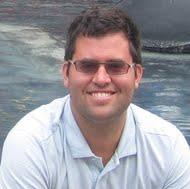
\includegraphics[height=1.25in]{mike.jpg}} & \\
  & \\
  & Michael Mulhearn \\
  & mulhearn@physics.ucdavis.edu \\
  & Physics 317 \\
  & \\
\end{tabular}
\vskip 0.5cm
\noindent
\textbf {Lectures:} M,W,F 2:10-3:00 PM in PHY 140
\begin{tabbing}
\hspace*{3em}\= \hspace*{5em} \= \kill % set the tabbings
\textbf {Lab:}    \> Section 1: \> M 3:10-6:00 PM in Roessler 152\\
                  \> Section 2: \> W 3:10-6:00 PM in Roessler 152\\
\end{tabbing}

\noindent
\begin{tabbing}
\hspace*{8em} \= \kill 
\textbf{Textbooks:} \> Lecture notes on passive electronics (course websites)\\
\>{\bf Practical Electronics for Inventors} by Scherz and Monk (Recommended)\\
\> {\bf The Art of Electronics} by Horowitz and Hill (Alternative)\\
\end{tabbing}

\noindent
\begin{tabbing}
\hspace*{8em} \= \kill 
\textbf{Lab Instructor:} \> Rahim Ullah (rrullah@ucdavis.edu) \\ 
\end{tabbing}

\noindent
\begin{tabbing}
\hspace*{8em}\= \hspace*{5em} \= \kill 
\textbf{Office Hours:}    \> Mulhearn: \> TBA \\
   \> Ullah: \> F 3:10-4:30 PM in Roessler 152 \\
\end{tabbing}

\noindent
\textbf {Course Description:}  
Experimental and theoretical study of important electronic circuits
involving analog and digital components.  Feedback, amplifiers,
oscillators, noise, integrated circuits, digital logic, timers,
analog-to-digital and digital-to-analog converters.\\

\noindent
\textbf{Midterm Exam:} TBA \\

\noindent
\textbf{Final Exam:} Mon, March, 14 2022 8:00 AM in Physics 140

\noindent
\textbf {Lab Safety:}\\
You should complete the online course for Electrical Safety at \\
{\tt http://safetyservices.ucdavis.edu/training/electrical-safety}.\\
You should also read your lab descriptions carefully, and ask your TA if you have any concerns about safety.\\

\newpage
\noindent
\textbf {Labs:}\\
The lab portion of this class is the most important.  You are expected
to attend every lab session.  You should come to each lab well
prepared, having read through the lab write-up ahead of time, with a
clear plan in mind.  A short write-up of each lab is due the following
week.  Your lab TA will clarify what should be included in each
write-up, the deadlines, grading criteria, and submission details.
Your lowest lab score will be dropped.  The lab instructor has office hours in the lab on Friday, which you can be used to finish labs you did not manage to finish during regular lab hours.\\

\noindent
\textbf{Homework:}\\
There will be approximately five homework assignments, based on the
lecture material.  Do not post the problems to internet forums.  To
minimize the effectiveness of cheating, homework scores will be based
solely on whether a legitimate attempt was made.  The best way to
prepare for the exams is to solve problems yourself or by actively
participating within a study group.  Always be prepared to explain
your work.  Homework and due dates will be posted on the course
website.\\

\noindent
\textbf {Grades:}\\
Final grades will be approximately $15\%$ Homework, $15\%$ Exams, and
$70\%$ lab write-ups.  Your worst lab score will be dropped.\\

\noindent
\textbf {COVID-19 Precautions and Accommodations:}\\
\noindent
Please review the information for students provided at:
\begin{quote}
{\tt https://campusready.ucdavis.edu/students-and-families}.
\end{quote}
Be ready to present your Daily Symptom Survey results at any in-person
activity, as we will be spot checking.  Do not attend in-person
activities without an approved status.

Your lowest lab score will be dropped.  In addition, you may submit
one lab assignment and two homework assignments late with no penalty
applied to the score.  This provides effectively two weeks of
accommodation which can handle downtime due to COVID-19.  If you miss
the midterm for a documented reason, your final exam score will be
used in place of your midterm score.  If you miss the final exam for a
documented reason, you will receive an Incomplete grade for the
course, until you can arrange to take a make-up exam.  Any further
accommodations should be pursued through the Student Disability Center
(SDC).

\newpage

\noindent
\textbf {Course Schedule}:\\
Here is the anticipated schedule for the course.  It may change as the
course progresses.\\

\noindent
\textbf {Lectures}:\\

\begin{tabular}{lll}
\textbf{Week} & \textbf{Dates} & \textbf{Topics} \\
\hline
1  & Jan 3,5,7       & Review (Asynchronous) \\
2  & Jan 10,12,14    & Review (Asynchronous) \\
3  & Jan 19,21       & Semiconductors, Transistors (Asynchronous)\\
4  & Jan 24,26,28    & Operational Amplifiers (Asynchronous)\\
5  & Jan 31, Feb 2,4 & Field Effect Transistors\\
6  & Feb 7,9,11      & Schmitt Trigger and Oscillators\\
7  & Feb 14,16,18    & Digital Logic \\
8  & Feb 21,23,25    & Synchronous Logic\\
9  & Feb 28, Mar 2,4 & PCBs, ASICs, FPGAs, CPUs\\
10 & Mar 7,9,11      & Review\\
\hline
\end{tabular}\\ \vskip 1cm

\noindent
\textbf {Labs}:\\

\begin{tabular}{lll}
\textbf{Week} & \textbf{Dates} & \textbf{Topics} \\
\hline
1  & Jan 3,5         & No Lab \\
2  & Jan 10,12       & No Lab \\ 
3  & Jan (17),19     & No Lab (Holiday)\\
4  & Jan 24,26       & Lab 1: Transistors\\
5  & Jan 31,Feb 2    & Lab 2: Op-Amps\\
6  & Feb 7,9         & Lab 3: Audio Amplifier\\
7  & Feb 14,16       & Lab 5: Schmitt Trigger and Oscillators\\
8  & Feb 21,23       & No Lab (Holiday)\\
9  & Feb 28, Mar 2   & Lab 6: Gates and Flip Flops\\
10 & Mar 7,9,11      & Lab 7: Combinatorics \\
\hline
\end{tabular} 

\end{document}

